\chapter{Tóm tắt lý thuyết}
\section{Mô hình động học phân tử chất khí}
\subsection{Chuyển động Brown}
\begin{itemize}
	\item Chuyển động Brown là chuyển động hỗn loạn, không ngừng, không theo quy luật, có quỹ đạo là đường gấp khúc bất kì của các hạt nhẹ trong chất lỏng và chất khí.
	\item Chuyển động Brown chứng tỏ các phân tử khí chuyển động hỗn loạn, không ngừng.
	\item Nhiệt độ càng cao, các phân tử khí chuyển động càng nhanh.
\end{itemize}
\subsection{Thuyết động học phân tử chất khí}
\begin{itemize}
	\item Chất khí được cấu tạo từ các phân tử có kích thước rất nhỏ so với khoảng cách trung bình giữa chúng.
	\item Các phân tử khí luôn chuyển động hỗn loạn, không ngừng. Nhiệt độ càng cao, các phân tử khí chuyển động càng nhanh.
	\item Trong quá trình chuyển động, các phân tử khí va chạm với thành bình chứa, gây ra áp suất lên thành bình.
\end{itemize}
\subsection{Lượng chất}
\begin{itemize}
	\item Đơn vị đo lượng chất là $\si{\mole}$.
	\item Mol là lượng chất trong đó chứa số phân tử (hoặc nguyên tử) bằng $N_A = \SI{6.022E23}{\mole^{-1}}$.	$N_A$ được gọi là số Avogadro.
	\item Một mẫu chất có khối lượng $m$, chứa $N$ phân tử thì có số mol là: $n=\dfrac{N}{N_A}=\dfrac{m}{M}$, trong đó
	$M$ (khối lượng mol) là khối lượng của 1 mol chất đó.
\end{itemize}
\section{Các định luật khí lí tưởng}
\subsection{Khí lí tưởng}
\begin{itemize}
	\item Khí lí tưởng là chất khí tuân theo đúng định luật Boyle và định luật Charles.
	\item Nội năng của khí lí tưởng chỉ phụ thuộc vào nhiệt độ.
\end{itemize}
\subsection{Định luật Boyle}
\begin{itemize}
	\item Ở nhiệt độ không đổi, áp suất của một khối lượng khí xác định tỉ lệ nghịch với thể tích	của nó.
	$$pV=\text{hằng số}\quad \text{hay}\quad p_1V_1=p_2$$
	\item Đồ thị biểu diễn sự phụ thuộc của áp suất theo thể tích khi nhiệt độ của khối khí không đổi được gọi là đường đẳng nhiệt.
	\begin{center}
		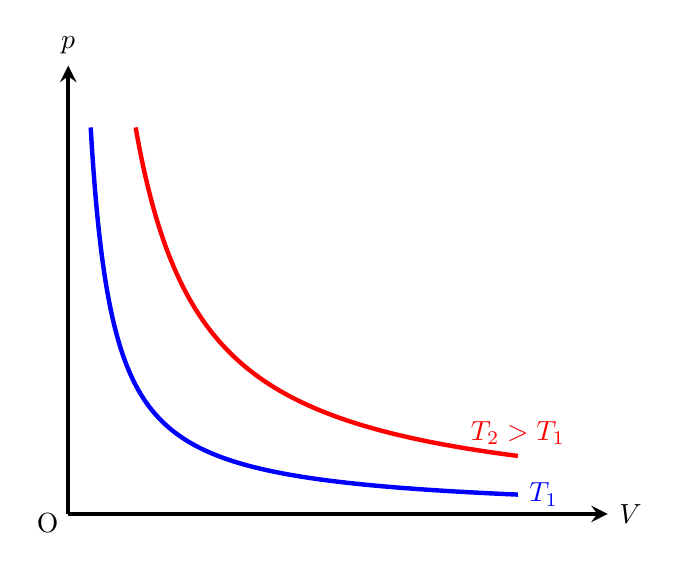
\begin{tikzpicture}  
			\begin{axis}[  ultra thick,
				xmin=0,  
				xmax=24,  
				xtick=\empty,
				ytick=\empty,
				ymin=0,  
				ymax=5.8, 
				samples=300,
				xticklabels=\empty,
				yticklabels=\empty,
				axis lines=center, 
				xlabel=$V$, 
				ylabel=$p$, 
				every axis y label/.style={at=(current axis.above origin),anchor=south},  
				every axis x label/.style={at=(current axis.right of origin),anchor=west},  ]
				\addplot [ultra thick, blue, smooth, domain=1:20] {5/x} node[right] {$T_1$}; 
				\addplot [ultra thick, red, smooth, domain=3:20] {15/x} node[above] {$T_2>T_1$}; 
			\end{axis}  
			\node[label={[below left]90:O}] at (0,0){};
		\end{tikzpicture}
	\end{center}
\end{itemize}
\subsection{Định luật Charles}
\begin{itemize}
	\item Ở áp suất không đổi, thể tích của một khối lượng khí xác định tỉ lệ thuận với nhiệt độ tuyệt đối của nó.
	$$\dfrac{V}{T}=\text{hằng số}\quad \text{hay}\quad \dfrac{V_1}{T_1}=\dfrac{V_2}{T_2}$$
	\item Đồ thị biểu diễn sự phụ thuộc của thể tích theo nhiệt độ tuyệt đối khi áp suất của khối khí không đổi được gọi là đường đẳng áp.
	\begin{center}
		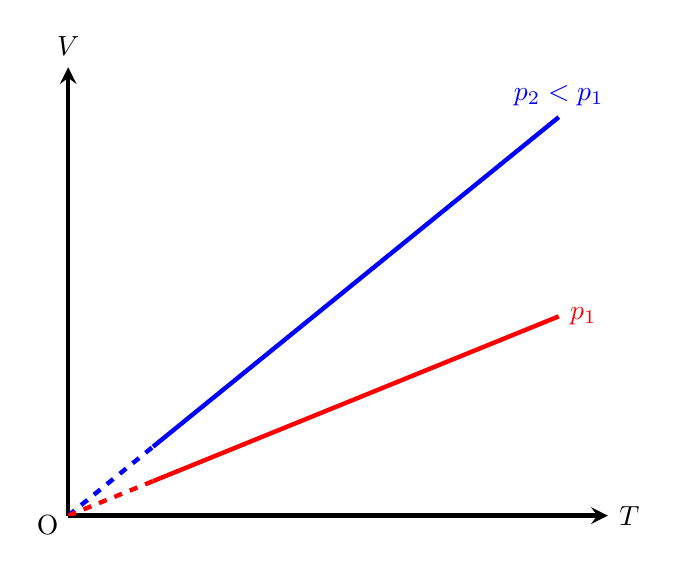
\begin{tikzpicture}  
			\begin{axis}[  ultra thick,
				xmin=0,  
				xmax=1100,  
				xtick=\empty,
				ytick=\empty,
				ymin=0,  
				ymax=900, 
				samples=300,
				xticklabels=\empty,
				yticklabels=\empty,
				axis lines=center, 
				xlabel=$T$, 
				ylabel=$V$, 
				every axis y label/.style={at=(current axis.above origin),anchor=south},  
				every axis x label/.style={at=(current axis.right of origin),anchor=west},  ]
				\addplot [ultra thick, blue, smooth,dashed, domain=0:173] {0.8*x}; 
				\addplot [ultra thick, blue, smooth, domain=173:1000] {0.8*x} node[above]{$p_2<p_1$}; 
				\addplot [ultra thick, red, smooth,dashed, domain=0:173] {0.4*x}; 
				\addplot [ultra thick, red, smooth, domain=173:1000] {0.4*x} node[right]{$p_1$};
			\end{axis}  
			\node[label={[below left]90:O}] at (0,0){};
		\end{tikzpicture}
	\end{center}
\end{itemize}
\subsection{Phương trình trạng thái của khí lí tưởng}
$$\dfrac{pV}{T}=nR\quad \text{hay}\quad \dfrac{p_1V_1}{T_1}=\dfrac{p_2V_2}{T_2}$$
Trong đó, $R\approx \SI{8.31}{\joule/\mole\cdot\kelvin} \approx\SI{0.082}{\dfrac{\liter\cdot atm}{\mole\cdot\kelvin}}$
là hằng số khí lí tưởng; $n$ là số mol khí.
\section{Áp suất và động năng của phân tử khí}
\subsection{Áp suất chất khí}
\begin{itemize}
	\item Áp suất khí tác dụng lên thành bình càng tăng khi các phân tử khí chuyển động nhiệt càng nhanh, khối lượng và mật độ phân tử khí càng lớn.
	\item Biểu thức tính áp suất chất khí tác dụng lên thành bình:
\end{itemize}
$$p=\dfrac{1}{3}\mu m\overline{v^2}=\dfrac{2}{3}\mu W_{\text{đ}}$$
trong đó:
\begin{itemize}
	\item $p$: áp suất khí tác dụng lên thành bình, đơn vị trong hệ SI là $\si{\newton/\meter^2}$;
	\item $\mu=\dfrac{N}{V}$: mật độ phân tử khí, đơn vị trong hệ SI là $\si{\meter^{-3}}$;
	\item $m$: khối lượng của một phân tử khí, đơn vị trong hệ SI là $\si{\kilogram}$;
	\item $\overline{v^2}$: trung bình của bình phương tốc độ, đơn vị trong hệ SI là $\si{\meter^2/\second^2}$;
	\item $W_{\text{đ}}$: động năng tịnh tiến trung bình của phân tử, đơn vị trong hệ SI là $\si{\joule}$.
\end{itemize}
\luuy{
Tốc độ căn quân phương $v_c=\sqrt{\overline{v^2}}$ \textbf{không phải} là tốc độ trung bình của các phân tử khí.
}
\subsection{Động năng tịnh tiến trung bình của phân tử khí}
Động năng tịnh tiến trung bình của phân tử khí tỉ lệ thuận với nhiệt độ tuyệt đối của khí.
$$W_{\text{đ}}=\dfrac{3}{2}kT.$$
Trong đó $k$ là hằng số Boltzmann: $k=\dfrac{R}{N_A}\approx\SI{1.38E-23}{\joule/\kelvin}$.
\subsection{Nội năng của khí lí tưởng đơn nguyên tử}
$$U=\dfrac{3}{2}nRT.$$